\documentclass{pssbmac}

%%%%%%%%%%%%%%%%%%%%%%%%%%%%%%%%%%%%%%%%%%%%%%%%%%%%%%%%%%%%%%%%%%%%%%%%
%% POR FAVOR, NÃO FAÇA MUDANÇAS NESSE PADRÃO QUE ACARRETEM  EM
%% ALTERAÇÃO NA FORMATAÇÃO FINAL DO TEXTO
%%%%%%%%%%%%%%%%%%%%%%%%%%%%%%%%%%%%%%%%%%%%%%%%%%%%%%%%%%%%%%%%%%%%%%%%

%%%%%%%%%%%%%%%%%%%%%%%%%%%%%%%%%%%%%%%%%%%%%%%%%%%%%%%%%%%%%%%%%%%%%%%%
% POR FAVOR, ESCOLHA CONFORME O CASO
%%%%%%%%%%%%%%%%%%%%%%%%%%%%%%%%%%%%%%%%%%%%%%%%%%%%%%%%%%%%%%%%%%%%%%%%
\usepackage[brazil]{babel} % texto em Português
%\usepackage[english]{babel} % texto em Inglês

%\usepackage[latin1]{inputenc} % acentuação em Português ISO-8859-1
\usepackage[utf8]{inputenc} % acentuação em Português UTF-8
%%%%%%%%%%%%%%%%%%%%%%%%%%%%%%%%%%%%%%%%%%%%%%%%%%%%%%%%%%%%%%%%%%%%%%%%


%%%%%%%%%%%%%%%%%%%%%%%%%%%%%%%%%%%%%%%%%%%%%%%%%%%%%%%%%%%%%%%%%%%%%%%%
%% POR FAVOR, NÃO ALTERAR
%%%%%%%%%%%%%%%%%%%%%%%%%%%%%%%%%%%%%%%%%%%%%%%%%%%%%%%%%%%%%%%%%%%%%%%%
\usepackage[T1]{fontenc}
\usepackage{float}
\usepackage{graphics}
\usepackage{graphicx}
\usepackage{epsfig}
\usepackage{indentfirst}
\usepackage{amsmath, amsfonts, amssymb, amsthm, mathtools}
\usepackage{url}
\usepackage{csquotes}
% Ambientes pré-definidos
\newtheorem{theorem}{Theorem}[section]
\newtheorem{lemma}{Lemma}[section]
\newtheorem{proposition}{Proposition}[section]
\newtheorem{definition}{Definition}[section]
\newtheorem{remark}{Remark}[section]
\newtheorem{corollary}{Corollary}[section]
\newtheorem{teorema}{Teorema}[section]
\newtheorem{lema}{Lema}[section]
\newtheorem{prop}{Proposi\c{c}\~ao}[section]
\newtheorem{defi}{Defini\c{c}\~ao}[section]
\newtheorem{obs}{Observa\c{c}\~ao}[section]
\newtheorem{cor}{Corol\'ario}[section]

% ref bibliográficas
\usepackage[backend=biber, style=numeric-comp%, maxnames=50
]{biblatex}
\addbibresource{refs.bib}
\DeclareTextFontCommand{\emph}{\boldmath\bfseries}
\DefineBibliographyStrings{brazil}{phdthesis = {Tese de doutorado}}
\DefineBibliographyStrings{brazil}{mathesis = {Disserta\c{c}\~{a}o de mestrado}}
\DefineBibliographyStrings{english}{mathesis = {Master dissertation}}
%%%%%%%%%%%%%%%%%%%%%%%%%%%%%%%%%%%%%%%%%%%%%%%%%%%%%%%%%%%%%%%%%%%%%%%%
\usepackage{booktabs}
\usepackage{adjustbox}

\begin{document}
{}{\
%%%%%%%%%%%%%%%%%%%%%%%%%%%%%%%%%%%%%%%%%%%%%%%%%%%%%%%%%%%%%%%%%%%%%%%%
% TÍTULO E AUTORAS(ES)
%%%%%%%%%%%%%%%%%%%%%%%%%%%%%%%%%%%%%%%%%%%%%%%%%%%%%%%%%%%%%%%%%%%%%%%%

\title{Uma comparação entre métodos baseados em images ou parâmetros escalares para a seleção de precondicionadores}

\author{
    {\large Michael Souza}\thanks{michael@ufc.br}, {\small UFC, Fortaleza, CE},  {\large Luiz Mariano Carvalho}\thanks{luizmc@ime.uerj.br}, {\small  UERJ, Rio de Janeiro, RJ}, \\
    {\large Douglas Augusto}\thanks{daa@fiocruz.br}, {\small FOC, Rio de Janeiro, RJ }, {\large Jairo Panetta}\thanks{jairo.panetta@gmail.com}, {\small ITA, São José dos Campos, SP}, \\
    {\large Paulo Goldfeld}\thanks{goldfeld@matematica.ufrj.br}, {\small UFRJ, Rio de Janeiro, RJ}, {\large José R. P. Rodrigues}\thanks{jrprodrigues@petrobras.com.br}, {\small CENPES/Petrobras}, \\ {\small Rio de Janeiro, RJ} \\
}
}
\criartitulo
%%%%%%%%%%%%%%%%%%%%%%%%%%%%%%%%%%%%%%%%%%%%%%%%%%%%%%%%%%%%%%%%%%%%%%%%


%%%%%%%%%%%%%%%%%%%%%%%%%%%%%%%%%%%%%%%%%%%%%%%%%%%%%%%%%%%%%%%%%%%%%%%%
% TEXTO
%%%%%%%%%%%%%%%%%%%%%%%%%%%%%%%%%%%%%%%%%%%%%%%%%%%%%%%%%%%%%%%%%%%%%%%%

\begin{abstract}
{\bf Resumo}. Em computação de alto desempenho (HPC), a solução eficiente de grandes sistemas lineares esparsos é fundamental, 
sendo os métodos iterativos a escolha predominante. No entanto, a performance desses métodos está ligada ao precondicionador
 escolhido. A natureza multifacetada das matrizes esparsas
torna difícil a prescrição universal de precondicionadores. Avançando em metodologias anteriores, esta pesquisa apresenta a representação da esparsidade de uma matrizes
 por meio de imagens RGB. Utilizando uma rede neural convolucional
(CNN), a tarefa de seleção do precondicionador se transforma em um problema de classificação
multi-classe. Testes extensivos em 126 matrizes da coleção SuiteSparse enfatizam a
adequação do modelo CNN, observando um aumento de 32\% na acurácia e uma redução de 25\%
no tempo de execução.

\noindent
{\bf Palavras-chave}. computação de alto desempenho (HPC), sistemas lineares esparsos,  métodos iterativos, escolha de precondicionadores,
 rede neural convolucional, classificação multi-classe
\end{abstract}

\section{Introdução}\label{sec:intro}

As simulações numéricas em, por exemplo, engenharia de reservatórios exigem 
a solução de grandes sistemas lineares com matrizes esparsas, ocupando em muitos casos mais de 50\% 
do tempo de computação 
\cite{gasparini21HybridParallelIterativeSparseLinearSolverFramework,gaganis2012machine}. 
Os métodos de Krylov são os solvers lineares preferidos nesse contexto. 
No entanto, seu sucesso depende da escolha de um precondicionador adequado, 
o que ainda é uma tarefa desafiadora, 
geralmente baseada em tentativa e erro ou na experiência do usuário 
\cite{saad2003iterative,scott2023introduction}.

Um precondicionador é uma matriz ou operador que modifica o sistema original 
para acelerar a convergência de solvers lineares iterativos. Vários fatores influenciam a 
eficácia do precondicionador, incluindo, entre outros, as diversas propriedades - estruturais ou matemáticas - da matriz esparsa,
a arquitetura computacional, as estruturas de dados empregadas 
\cite{benzi2002preconditioning,bell2008efficient}. 
Neste trabalho, abordaremos apenas o primeiro desses fatores.

Propor uma representação adequada para matrizes esparsas quando da sugestão de 
precondicionadores é um desafio, principalmente devido aos requisitos de escalabilidade. 
Para sistemas esparsos grandes, o ideal é que a complexidade computacional seja linear 
em relação ao número de elementos não nulos. Essa restrição decorre da necessidade de 
manter a eficiência à medida que o tamanho do sistema aumenta, o que é comum em, por exemplo, 
simulações de reservatórios ou em dinâmica de fluidos computacional. 
A dificuldade em obter representações compactas está em capturar as propriedades 
da matriz que mais influenciam o desempenho dos precondicionadores dentro 
dessa restrição de complexidade linear.

Entre os atributos da matriz que influenciam a escolha dos precondicionadores, 
podemos destacar a ordem da matriz, seus autovalores e valores singulares, 
o número de condicionamento, o padrão de esparsidade, a densidade e a dominância diagonal, 
entre outros.  Com a exceção do padrão de esparsidade, esses atributos são numéricos. A esparsidade
encapsula atributos topológicos sobre a conexão entre os elementos não nulos da matriz. 
Embora alguns atributos escalares, como a largura de banda e o número de elementos diferentes 
de zero, forneçam informações sobre padrões complexos de esparsidade, 
sua sensibilidade é baixa. Essa característica dificulta a obtenção de 
uma representação numérica adequada para a esparsidade. 

Embora não seja o único fator determinante, o padrão de esparsidade afeta o 
nível de paralelismo possível tanto na aplicação quanto na construção de precondicionadores 
como ILU($k$) \cite{Meijerink1977AnIS, saad2003iterative}. No método multigrid algébrico (AMG),
os operadores grosseiros codificam a esparsidade e os valores numéricos para criar 
uma aproximação multinível do sistema \cite{stuben2001AReview}. Dependendo do padrão 
de esparsidade, até mesmo métodos diretos podem ser aplicáveis para resolver 
problemas esparsos \cite{Davis2016ASO}.

Neste trabalho, exploramos técnicas de aprendizagem profunda (AP) para obter 
automaticamente representações compactas de matrizes esparsas para selecionar 
precondicionadores. Ampliando a abordagem de Yamada et al. \cite{yamada2018preconditioner}, 
usamos imagens RGB para codificar espacialmente os padrões de esparsidade, 
facilitando a análise orientada por dados para aumentar a eficiência dos solvers lineares. 
Diferentemente do trabalho de Yamada, nossa metodologia incorpora a classificação 
de vários rótulos para identificar uma gama de precondicionadores adequados 
para uma determinada matriz esparsa. Para processar as representações baseadas 
em imagens, empregamos uma rede neural convolucional (CNN) \cite{li2022survey}.

Nossas contribuições são as seguintes: 
 \begin{description}  
\item [Modelo multi-rótulo:] Em tarefas de classificação convencionais, 
uma matriz esparsa é frequentemente mapeada para apenas um precondicionador. 
Entretanto, em nosso conjunto de dados, aproximadamente 20\% das matrizes exibem 
vários precondicionadores ideais. Com base na pesquisa de Yamada et al.
\cite{yamada2018preconditioner}, nós não seguimos a abordagem de mapeamento de um para um. 
Ao adotar uma estrutura com vários rótulos, permitimos atribuir vários precondicionadores 
a uma única matriz, lidando melhor com casos em que vários precondicionadores têm desempenho 
semelhante.  
\item [Modelos escalares versus modelos baseados em imagens:] Comparamos modelos escalares 
e com alguns baseados em imagens. Nossa pesquisa também introduziu um modelo misto que combina 
os dois atributos, transformando os atributos baseados em imagem em um formato 
vetorial (\emph{achatamento}) e, posteriormente, integrando-os à tabela de atributos escalares.  
\item[Resultados promissores:] Em nossa pesquisa inicial, os modelos baseados em imagens 
superam os modelos baseados em escalas na seleção do precondicionador. Eles mostram 
uma probabilidade 32\% maior de sugestão de precondicionador ideal e uma chance 26\% maior 
de baixo impacto computacional quando não se escolhe o precondicionador ideal. Esses 
resultados destacam a eficiência e a eficácia superiores dos modelos baseados em imagens.  
\end{description}

Esta contribuição resume um trabalho em desenvolvimento que 
se encontra disponível em \cite{souza2023}; vários detalhes omitidos aqui, 
dado o limite do número de páginas, podem ser encontrados neste trabalho.
O restante deste artigo está assim estruturado: a Seção \ref{sec:related} 
analisa a literatura relevante, a Seção \ref{sec:method} descreve nossa metodologia, 
a Seção \ref{sec:results} discute os resultados empíricos e a Seção \ref{sec:conclusions} 
conclui o artigo, destacando sua importância e sugerindo futuras direções de pesquisa.

\section{Trabalhos relacionados}\label{sec:related}

O potencial da aprendizagem profunda (AP) para discernir padrões complexos e 
facilitar a tomada de decisões orientada por dados foi reconhecido 
como uma solução eficaz para vários desafios na computação de alto desempenho 
aplicada à solução de sistemas lineares 
\cite{falch2017machine,tuncer2017diagnosing,memeti2019using}.

Uma área de aplicação da AP é a seleção automática da estrutura de dados 
para o armazenamento de matrizes esparsas. Sedaghati et al. \cite{sedaghati2015automatic}
usaram algoritmos de árvore de decisão para automatizar a seleção do formato de 
armazenamento com base nas propriedades da matriz. Nisa et al. \cite{nisa2018effective} 
aplicaram técnicas de aprendizado de máquina para prever os formatos de 
armazenamento mais adequados para GPUs. A importância de sincronizar a estrutura de dados 
de armazenamento com a eficiência computacional também é destacada na pesquisa de 
Barreda et al. \cite{barreda2020performance} e Cui et al. \cite{cui2016code} 
que exploram melhorias de desempenho em diferentes plataformas de computação.

Outra aplicação de AP notável envolve (\emph{autoajuste}) de solvers lineares. 
Por exemplo, Peairs e Chen \cite{peairs2011using} utilizaram uma estratégia de 
aprendizagem por reforço para determinar os parâmetros de reinício ideais para o 
GMRES. Bhowmick et al. \cite{bhowmick2006application} aplicaram a AP para selecionar 
os melhores solvers para sistemas lineares esparsos em tempo de execução, 
adaptando-se aos dados e à arquitetura computacional disponível. 
Dufrechou et al. \cite{dufrechou2019automatic} empregaram técnicas de AP 
para prever o solver ideal para um sistema linear específico, concentrando-se 
em situações em que um número limitado de sistemas triangulares é resolvido para a 
mesma matriz. 
Em outra abordagem, Funk et al. \cite{funk2022prediction} apresentaram uma técnica de 
aprendizagem profunda para identificar o solver iterativo ideal para 
um determinado sistema linear esparso, obtendo uma acurácia de classificação de 60\%.

Uma tendência crescente na AP é o uso de redes neurais para acelerar os 
operações de álgebra linear. Cui et al. \cite{cui2016code} empregaram um sistema de 
AP para prever a melhor implementação da multiplicação matriz-vetor (SpMV) para uma 
determinada matriz. G{\"o}tz e Anzt \cite{gotz2018machine} introduziram 
uma rede neural convolucional (CNN) para detectar estruturas de blocos em 
padrões de esparsidade de matriz. Em uma abordagem diferente, 
Ackmann et al. \cite{ackmann2020machine} propuseram o uso de uma 
rede neural feed-forward como precondicionador. Taghibakhshi et al. 
\cite{taghibakhshi2021optimization} introduziram um método inovador usando 
um agente de aprendizagem por reforço baseado em redes neurais de grafos (GNNs) 
para construir espaços grosseiros em uma abordagem multigrid. 

Embora a AP tenha otimizado substancialmente vários aspectos da álgebra linear computacional,
seu potencial na seleção de precondicionadores merece ser mais explorado. 
Este trabalho é uma contribuição nessa direção.

\section{Metodologia}\label{sec:method}

Propomos codificar a esparsidade da matriz e alguns atributos facilmente 
computáveis como imagens RGB. Essa representação geométrica é uma descrição compacta 
e adequada da estrutura da matriz subjacente. Para comprovar essa afirmação, 
realizamos experimentos comparando modelos de AP treinados em atributos de 
matriz escalar com aqueles treinados em imagens. Em ambos os cenários, o 
objetivo principal é a seleção ideal de precondicionadores para minimizar o tempo de 
convergência dos solucionadores lineares.

Para este estudo, empregamos 126 matrizes simétricas, 
não diagonais e positivo-definidas da coleção de matrizes SuiteSparse usando a
biblioteca \texttt{ssgetpy} \cite{kolodziej2019suitesparse,ssgetpy}. 

Empregamos um conjunto de parâmetros escalares para caracterizar 
as matrizes, ver Tabela \ref{tab:scalar_features}.
Entre esses parâmetros, o número da condicionamento foi calculado usando a 
função \texttt{condest} do MATLAB, enquanto os menores e maiores autovalores 
foram obtidos por meio da função \texttt{eigs} com as opções \texttt{smallestabs} e 
\texttt{largestabs}, respectivamente \cite{matlab}. 
Embora o número de condicionamento e os autovalores sejam informativos, 
eles são computacionalmente caros. Em contrapartida, 
nossa abordagem baseada em imagens oferece uma alternativa igualmente informativa, 
porém mais eficiente.

\begin{table}
    \centering
    \caption{Propriedades Escalares.}
    \label{tab:scalar_features}
\begin{tabular}{@{}p{2cm}p{9cm}@{}}
    \toprule
    \textbf{Nome} &  \multicolumn{1}{c}{\textbf{Definição}} \\
    \midrule
    Densidade & Número de elementos diferentes de zero dividido pelo número total de elementos. \\
    N& Número de linhas. \\
    NNZ & Número de elementos diferentes de zero. \\
    RowNNZ & Número médio de elementos diferentes de zero por linha. \\
    Condest & Estimativa do número de condicionamento da matriz, com a norma 1. \\
    MinEigs & Estimativa do menor autovalor da matriz. \\
    MaxEigs & Estimativa do maior autovalor da matriz. \\
    DDom & Percentagem das linhas dominadas diagonalmente. Se $D$ for a matriz diagonal extraída de $A$, $B = A - D$, $S = \{ i: |D_{ii}| > \sum_j{|B_{ij}|}\}$, então $\text{DDom} = \frac{|S|}{N}.$\\
    DDeg & Razão mínima entre o valor absoluto do elemento diagonal e a soma das entradas não diagonais. $\text{DDeg} = \min_{i}\frac{|D_{ii}|}{\sum_j{|B_{ij}|}}$.\\
    \bottomrule
\end{tabular}
\end{table}

A Tabela \ref{tab:scalar_features_summary} apresenta um resumo estatístico de propriedades escalares das matrizes analisadas. 
Apesar de todas as matrizes serem simétricas e  positivo-definidas (SPD), o menor valor próprio estimado é 
$-3,60$. Essa contradição decorre da acurácia limitada da função \texttt{eigs}, que pode não calcular com 
corretamente o menor autovalor para matrizes específicas. 
Embora o número de condicionamento de uma matriz SPD seja definido por seus autovalores extremos, os atributos que 
empregamos são estimativas, o que os torna não redundantes.
\begin{table}
    \caption{Propriedades das Matrizes.}
    \label{tab:scalar_features_summary}
    \begin{adjustbox}{width=\textwidth}
    \begin{tabular}{lrrrrrrrrr}
    \toprule
    & N & NNZ & Densidade & RowNNZ& MaxEigs & MinEigs & Condest & DDom & DDeg \\
    \midrule
    \textbf{média} & 4.1E+04& 6.1E+05& 1.1E-02& 2.5E+01& 1.9E+13& 9.6E+07& 1.2E+17& 1.4E-01& 2.0E-01\\
    \textbf{std} & 1.2E+05& 1.2E+06& 1.8E-02& 3.8E+01& 1.3E+14& 7.3E+08& 9.1E+17& 3.1E-01& 3.6E-01\\
    \textbf{mín} & 1.0E+02& 5.9E+02& 5.0E-06& 2.9E+00& 9.8E-13& -3.6E+00& 3.6E+00& 0.00& 7.9E-15\\
    \textbf{25\%} & 1.1E+03& 1.9E+04& 3.8E-04& 6.8E+00& 9.7E+00& 1.5E-04& 4.5E+03& 0.00& 8.5E-04\\
    \textbf{50\%} & 8.6E+03& 1.3E+05& 3.8E-03& 1.6E+01& 2.9E+04& 2.0E-01& 3.9E+06& 0.00& 4.8E-03\\
    \textbf{75\%} & 2.9E+04& 5.6E+05& 1.3E-02& 2.6E+01& 5.7E+08& 2.8E+00& 1.5E+09& 2.6E-03& 2.2E-01\\
    \textbf{máx} & 1.0E+06& 5.5E+06& 9.1E-02& 3.6E+02& 1.1E+15& 5.8E+09& 9.4E+18& 1.0E+00& 1.8E+00\\
    \bottomrule
    \end{tabular}
    \end{adjustbox}
\end{table}

Para representar visualmente as propriedade da matriz, criamos um conjunto de dados de imagem com base 
no método proposto por Yamada et al. \cite{yamada2018preconditioner}. Cada matriz \( A \) é particionada 
em blocos \( A_{ij} \) de dimensão \( b \approx N / m \), em que \( N \) é a dimensão da matriz e $m$ é a 
resolução da imagem. Esses blocos são representados como pixels \( p_{ij} \) em uma imagem de \( m \times m \) pixels.
Geramos quatro conjuntos de imagens com \( m \in \{32, 64, 128, 256\}\).

Cada pixel \( p_{ij} \) consiste em três componentes alinhados com os canais RGB: vermelho, verde e azul. 
O canal vermelho captura a magnitude dos elementos diferentes de zero no bloco da matriz, 
o azul incorpora as dimensões da matriz e o verde transmite a densidade do bloco. 
Como resultado, as características distintas de cada matriz são visualmente representadas, 
com os atributos de cada bloco influenciando a cor do pixel correspondente. 

Denotaremos os canais vermelho, verde e azul do pixel $p_{ij}$ como $R_{ij}$, $G_{ij}$ e $B_{ij}$, respectivamente. 
O intervalo dos componentes do pixel é limitado de 0 a 255. Essa restrição e a necessidade de 
uma representação geral de matrizes heterogêneas exigem um esquema de codificação cuidadoso. 
Agora descrevemos a transformação da matriz em uma imagem:

\begin{description}
	\item[Canal Azul:] O canal azul tem o mesmo valor para todos os pixels, dado por
	$$B_{ij} = \left\lfloor\frac{N - N_{\min}}{N_{\max}  - N_{\min}}\times 255\right\rfloor,~i,j=1,\ldots,m,$$
	em que $N$ é a ordem da matriz, $N_{\min}$ e $N_{\max}$ são as ordens mínima e máxima de todas as matrizes 
    no conjunto de dados, respectivamente.
	
	\item[Canal Verde:] O valor do canal verde, \( G_{ij} \), é a densidade de elementos diferentes de zero 
    em um determinado bloco de matriz. Ele é definido como:
\[ G_{ij} = \left\lfloor\frac{NNZ_{ij}}{b^{2}}\times 255\right\rfloor \]
em que \( \operatorname{NNZ}_{ij} \) representa a contagem de elementos diferentes de zero no bloco
\( A_{ij} \) e \( b \) denota a ordem do bloco.

	\item[Canal Vermelho:] Para representar a magnitude média dos elementos diferentes de zero 
    nos blocos de uma matriz esparsa, primeiro ajustamos ou “polarizamos” seus elementos diferentes de zero.  
    Isso é feito para garantir que todos os valores sejam maiores que zero. Especificamente, 
    para qualquer elemento diferente de zero \(a\) na matriz \(A\), seu valor enviesado 
    \(v(a)\) é dado por $v(a) = a - \min(A) + 1,$ em que $\min(A)$ é o elemento mínimo de $A$.

A próxima etapa é calcular a média desses valores enviesados para cada bloco da matriz. 
Vamos chamar essa média de \( \gamma_{ij} \) para o bloco \(A_{ij}\). Se a diferença entre os valores 
máximo e mínimo de toda a matriz for igual ou inferior a 255, calcularemos a média dos valores enviesados
dentro do bloco. Se a diferença for maior que 255, calculamos o logaritmo de base 2 dos valores enviesados
antes de calcular a média. Esse método lida com eficiência com blocos de valores amplamente variáveis, 
mudando o foco da magnitude para a ordem de magnitude.

A fórmula é a seguinte:
\[\gamma_{ij} = \frac{\sum_{a \in A_{ij}} v(a)}{NNZ_{ij}},\]
quando a diferença entre os valores máximo e mínimo for igual ou inferior a 255, e 
\[\gamma_{ij} = \frac{\sum_{a \in A_{ij}} \log_2 v(a)}{NNZ_{ij}},\]
caso contrário.

Por fim, com as médias de bloco em mãos, podemos definir o valor $R_{ij}$ como a 
normalização da média de bloco com relação ao intervalo geral de médias de bloco, ou seja 
\[R_{ij} = \left\lfloor \frac{\gamma_{ij} - \min(\gamma)} {\max(\gamma) - \min(\gamma)} \times 255 \right\rfloor\]
\end{description}

A Figura \ref{fig:matrix_to_image} ilustra a conversão de uma matriz de $20 \times 20$ em 
uma imagem de $5\times 5$ pixels, com \(m=5\). Aqui, cada pixel na imagem corresponde a um bloco 
de $4 \times 4$ da matriz.
\begin{figure}[ht]
    \centering
    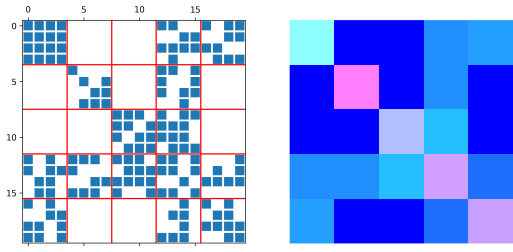
\includegraphics[width=0.8\textwidth]{Figuras/figure01}
    \caption{Representação baseada em imagem de uma matriz de $20 \times 20$. A matriz é dividida em blocos $ 5 \times 5$ e os valores das propriedades são codificados nos canais de cores RGB}.
    \label{fig:matrix_to_image}entradas
\end{figure}
O conjunto completo de dados de imagem pode ser acessado e baixado do repositório do GitHub \cite{ImagePrecGitHub}.

A representação da esparsidade como imagens captura naturalmente as informações topológicas, 
codificando-as em relações geométricas, que são mais difíceis de serem obtidas com representações escalares. 
Para destacar a importância dessas nuances geométricas nas representações de imagens, geramos um banco de 
dados misto que combina atributos escalares e imagens. Nessa variação, as imagens RGB de $m \times m$ pixels 
foram colocadas em vetores com  $3m^2$ entradas. Concatenamos os vetores achatados com os atributos escalares, 
combinando assim as duas representações.

Esse processo gerou quatro conjuntos de atributos escalares estendidos, correspondentes a cada 
$m \in \{32, 64, 128, 256\}$. Para gerenciar o aumento da dimensionalidade e reter os aspectos mais
informativos desses atributos estendidos, usamos a análise de componentes principais (PCA), 
capturando 99\% da variação nos dados \cite{guyon2006introduction}.


\section{Resultados}\label{sec:results}próprios
\section{Conclusões}\label{sec:conclusions}



Equações inseridas no trabalho completo devem ser enumeradas sequencialmente e à direita no texto, por exemplo
\begin{equation}
\frac{\partial u}{\partial t}-\Delta u = f, \quad  \mathrm{em} \; \Omega. \label{Calor}
\end{equation}
Consulte o arquivo \verb!.tex! para mais detalhes sobre o código-fonte gerador da equação \eqref{Calor}.

\section{Tabelas e Figuras}

As(os) autoras(es) podem inserir figuras e tabelas no artigo. Elas devem estar dispostas próximas de suas referências no texto.

\subsection{Inserção de Tabelas}

A inserção de tabela deve ser feita com o ambiente \verb!table!, sendo enumerada, disposta horizontalmente centralizada, próxima de sua referência no texto, e a legenda imediatamente acima dela. Por exemplo, consulte a Tabela \ref{tabela01}.

\begin{table}[H]
\caption{ {\small Categorias dos trabalhos.}}
\centering
\begin{tabular}{ccc}
\hline
Categoria do trabalho  & Número de páginas & Tipo do trabalho\\ \hline
1          & 2  & $A$, $B$ e $C$    \\
2          & entre 5 e 7  & apenas $C$ \\
\hline
\end{tabular}\label{tabela01}
\end{table}

\subsection{Inserção de Figuras}

A inserção de figura deve ser feita com o ambiente \verb!figure!, ela deve estar enumerada, disposta horizontalmente centralizada, próxima de sua referência no texto, e legenda imediatamente abaixo dela. \emph{Quando não própria, deve-se indicar/referências a fonte.} Por exemplo, consulte a Figura \ref{figura01}.

\begin{figure}[H]
\centering

\includegraphics[width=.7\textwidth]{ex_fig}
\caption{ {\small Exemplo de imagem. Fonte: indicar.}}
\label{figura01}
\end{figure}

\section{Sobre as Referências Bibliográficas}

As referências bibliográficas devem ser inseridas conforme especificado neste padrão, 
sendo que serão automaticamente geradas em ordem alfabética pelo sobrenome do primeiro autor. 
Este {\it template} fornece suporte para a inserção de referências bibliográficas com o Bib\LaTeX{}. 
Os dados de cada referência do trabalho devem ser adicionados no arquivo \verb+refs.bib+ e a
 indicação da referência no texto deve ser inserida com o comando \verb+\cite+. 
 Seguem alguns exemplos de referências: livro \cite{Boldrini}, artigos publicados em periódicos 
 \cite{Contiero,Cuminato}, capítulo de livro \cite{daSilva}, dissertação de mestrado \cite{Diniz}, 
 tese de doutorado \cite{Mallet}, livro publicado dentro de uma série \cite{Gomes}, 
 trabalho publicado em anais de eventos \cite{Santos}, {\it website} e outros \cite{CNMAC}. 
 Por padrão, os nomes de todos os autores da obra citada aparecem na bibliografia. 
 Para obras com mais de três autores, é também possível indicar apenas o nome do primeiro autor, 
 seguido da expressão et al. Para implementar essa alternativa, basta remover ``\verb+,maxnames=50+'' 
 do comando correspondente do código-fonte. Sempre que disponível forneça o DOI, ISBN ou ISSN, conforme o caso.

\section{Considerações Finais}

Esta seção é reservada às principais conclusões e considerações finais do trabalho.

\section*{Agradecimentos (opcional)}

Seção reservada aos agradecimentos dos autores, caso for pertinente. Por exemplo, agradecimento a fomentos. Se os autores optarem pela inclusão de Agradecimentos, a palavra ``(opcional)'' deve ser removida do título da seção. Esta seção não é numerada e deve ser disposta entre a última seção do corpo do texto e as Referências.


%%%%%%%%%%%%%%%%%%%%%%%%%%%%%%%%%%%%%%%%%%%%%%%%%%%%%%%%%%%%%%%%%%%%%%%%
% REFS BIBLIOGRÁFICAS
% POR FAVOR, NÃO ALTERAR
%%%%%%%%%%%%%%%%%%%%%%%%%%%%%%%%%%%%%%%%%%%%%%%%%%%%%%%%%%%%%%%%%%%%%%%%
\printbibliography
%%%%%%%%%%%%%%%%%%%%%%%%%%%%%%%%%%%%%%%%%%%%%%%%%%%%%%%%%%%%%%%%%%%%%%%%

\end{document}




